\section{A Bosch type theorem for the reciprocal Xi function}\label{ch:boschB}

\label{bs:sec:intro}The observation that closes Section~\ref{ch:boschA} becomes a theorem through an elasticity criterion (Theorem~\ref{bs:thm:crit}). Applied to $\varphi(s)=\xi(\frac12)/\xi(\frac12+\sqrt s)$ it gives a Bosch type theorem for $\varphi(x^{1/\beta})$ (Theorem~\ref{bs:thm:power}), and the same elasticity identifies the Thorin measure of $\varphi(s^p)$ (Theorem~\ref{bs:thm:ggc}); the positivity of its density is where the Riemann problem now sits.

The notation is that of Section~\ref{ch:boschA}: the clock $\varphi$ is a function of $s$, and $W$ is the Mellin variable with $\E W^z=\Xi(0)/\Xi(z)$, not the heat trace $W(t)$ of Section~\ref{ch:heat}. The numerical checks are made by \texttt{code\_bosch/\allowbreak verify\_bosch\_xi\_v7.py} in the repository and documented in \texttt{code/\allowbreak README.md}; the checks confirm formulas and constants and prove nothing.

\subsection{The elasticity criterion}\label{bs:sec:crit}

\label{bs:sec:facts}We use HCM as defined in Section~\ref{bh:sec:bosch}, with the facts (F1) to (F7) listed there, above all Bondesson's representation~\eqref{bs:eq:bond} \cite[(5.2.3) and Theorem 5.3.1]{Bondesson}. Throughout, $\Om=\C\setminus(-\infty,0]$, $\C^+=\{\Im x>0\}$, and a Pick function is an analytic map $\C^+\to\overline{\C^+}$. For a GGC with Laplace transform $h$, drift $b\ge0$ and Thorin measure $U$, in the sense of~\eqref{eq:ch3:ggc}, $-h'/h=b+\int U(dt)/(x+t)$ is a Stieltjes function. We also need two facts about complete Bernstein functions \cite[Theorem 6.2]{boSSV}: a function $f$ on $(0,\infty)$ is complete Bernstein if and only if $f\ge0$ on $(0,\infty)$ and $f$ continues to a Pick function analytic on $\Om$, and then $f(x)/x$ is a Stieltjes function.

The elasticity criterion below restates~\eqref{bs:eq:bond} as a Pick function condition, of the kind through which Bosch verifies HCM \cite[Section 2.2]{boBosch}.

\begin{definition}
For $h$ analytic and zero free on $\Om$ and positive on $(0,\infty)$, let $\log h$ be the branch that is real on $(0,\infty)$ and define the elasticity $\varepsilon_h(x)=-xh'(x)/h(x)$. In logarithmic coordinates $x=e^z$ one has $\varepsilon_h(e^z)=-\frac{d}{dz}\log h(e^z)$.
\end{definition}

\begin{theorem}\label{bs:thm:crit}
Let $h>0$ on $(0,\infty)$. Then $h$ is HCM if and only if $h$ continues to a zero free analytic function on $\Om$ and $\varepsilon_h$ is a Pick function, that is $\Im\varepsilon_h(x)\ge0$ for $\Im x>0$.
\end{theorem}

\begin{proof}
Necessity. By~\eqref{bs:eq:bond}, $h$ is zero free and analytic on $\Om$, and its elasticity is
\[
\varepsilon_h(x)=1-r+b_1x+\int\frac{x}{x+t}\,\Gamma_1(dt)-\frac{b_2}{x}-\int\frac{\Gamma_2(dt)}{1+tx}.
\]
For $\Im x>0$ each term has nonnegative imaginary part, for instance $\Im\frac{x}{x+t}=\frac{t\Im x}{|x+t|^2}$.

Sufficiency. Fix $u>0$. The principal branch $y(w)=\operatorname{arccosh}(w/2)$ maps $\C\setminus(-\infty,2]$ conformally onto the half strip $S=\{\Re y>0,\ |\Im y|<\pi\}$, and $w=2\cosh y$. For $y\in S$ both $ue^{y}$ and $ue^{-y}$ lie in $\Om$, so
\[
F(w)=-\log h\bigl(ue^{y(w)}\bigr)-\log h\bigl(ue^{-y(w)}\bigr)
\]
is analytic on $\C\setminus(-\infty,2]$ and real on $(2,\infty)$, and $e^{-F(w)}$ is the pair function. Let $\Im w>0$, so $y=\varrho+i\theta$ with $\varrho>0$ and $\theta\in(0,\pi)$. Put $r_1=ue^{\varrho}>r_2=ue^{-\varrho}$. Since $\log h(\bar x)=\overline{\log h(x)}$,
\[
\Im F(w)=-\Im\log h(r_1e^{i\theta})+\Im\log h(r_2e^{i\theta}).
\]
Along the ray, $\partial_r\Im\log h(re^{i\theta})=\Im\bigl(e^{i\theta}h'/h\bigr)=-r^{-1}\Im\varepsilon_h(re^{i\theta})\le0$, so $\Im F(w)\ge0$. Thus $F$ is a Pick function that continues analytically across $(2,\infty)$, where it is real. By the Nevanlinna representation $F(w)=a+bw+\int(\frac1{t-w}-\frac t{1+t^2})\sigma(dt)$ with $b\ge0$ and $\sigma\ge0$ carried by $(-\infty,2]$. Hence for $w>2$,
\[
F'(w)=b+\int_{(-\infty,2]}\frac{\sigma(dt)}{(w-t)^2}=b+\int_{(-\infty,2]}\int_0^\infty\lambda e^{-\lambda(w-t)}\,d\lambda\,\sigma(dt),
\]
which is completely monotone. A function whose derivative is completely monotone is a Bernstein function up to an additive constant, and $e^{-F}$ is then completely monotone. So every pair function is completely monotone and $h$ is HCM.
\end{proof}

The two conditions play different roles. Analyticity without zeros is global and rigid: a single zero or pole of $h$ anywhere off the negative axis destroys HCM, however small its effect on the real line. The Pick condition is local and quantitative: it can fail along a ray without any singularity.

\subsection{Bosch's theorem from the criterion}\label{bs:sec:bosch}

Bosch's variable $T_\alpha=(Z_\alpha/\tilde Z_\alpha)^\alpha$, $0<\alpha<1$, of Section~\ref{bh:sec:bosch} has the density $\sin(\pi\alpha)/(\pi\alpha(t^2+2t\cos\pi\alpha+1))$ of a half Cauchy law with drift. Let $c=\cos\pi\alpha$ and $q=1/|\beta|$, half the $q$ of~\eqref{bh:eq:pair}. Since $T_\alpha\stackrel{d}{=}1/T_\alpha$ we may take $\beta>0$. The density of $T_\alpha^\beta$ is proportional to
\[
h(x)=\frac{x^{q-1}}{D(x)},\qquad D(x)=x^{2q}+2cx^q+1=(x^q+e^{i\pi\alpha})(x^q+e^{-i\pi\alpha}).
\]

\begin{theorem}[Bosch {\cite[Theorem 1.2]{boBosch}}]\label{bs:thm:bosch}
$h$ is HCM if and only if $\alpha\le1/2$ and $q\le1-\alpha$.
\end{theorem}

\begin{proof}
Zeros. For $x\in\Om$ the value $x^q$ ranges over the sector $|\arg|<q\pi$. The zeros of $D$ satisfy $x^q=e^{\pm i(1-\alpha)\pi}$, so $D$ is zero free on $\Om$ if and only if $q\le1-\alpha$.

Elasticity. For $x=re^{i\theta}$ with $0<\theta<\pi$ write $x^q=Re^{i\omega}$ with $R=r^q$ and $\omega=q\theta\in(0,q\pi)$. Then $\varepsilon_h=1-q+xD'(x)/D(x)$ and $\Im\varepsilon_h=qR\,\partial_R\arg D$. A direct computation of $\Im(\partial_RD\cdot\overline D)$ gives
\begin{equation}\label{bs:eq:boschel}
\Im\varepsilon_h(x)=\frac{2qR\sin\omega\,\bigl(c(1+R^2)+2R\cos\omega\bigr)}{|D(x)|^2}.
\end{equation}
If $\alpha\le1/2$ and $q\le1-\alpha$ then $c\ge0$ and $\cos\omega\ge\cos((1-\alpha)\pi)=-c$, so, using $1+R^2\ge2R$, the bracket is at least $2R(c+\cos\omega)\ge0$. Theorem~\ref{bs:thm:crit} gives HCM. If $\alpha>1/2$ then $c<0$ and the bracket tends to $c<0$ as $R\to0$, so $\varepsilon_h$ is not Pick. If $q>1-\alpha$ then $h$ has poles in $\Om$. In both cases Theorem~\ref{bs:thm:crit} rules out HCM.
\end{proof}

In terms of $\beta$, the theorem says that the density of $T_\alpha^\beta$ is HCM if and only if $\alpha\le1/2$ and $|\beta|\ge1/(1-\alpha)$. For the half Cauchy variable, $\alpha=1/2$, the threshold is $|\beta|\ge2$; there $c=0$ and~\eqref{bs:eq:boschel} reduces to $\Im\varepsilon_h=4qR^2\sin\omega\cos\omega/|D|^2$, which is nonnegative for every $\omega\in(0,q\pi)$ exactly when $q\le1/2$. So the half Cauchy threshold is the condition $\omega\le\pi/2$, equivalently that the zeros $x=e^{\pm i\pi/(2q)}$ of $1+x^{2q}$ stay on or beyond the cut.

\subsection{The Riemann analogue}\label{bs:sec:xi}

As in Section~\ref{bh:sec:dict}, $\gamma$ runs over the zeros of $\Xi(z)=\xi(1/2+iz)$ with $\Re\gamma>0$, counted with multiplicity; the nonreal ones come in conjugate pairs $\gamma,\bar\gamma$. By~\eqref{eq:ch2:hadamard}, unconditionally,
\[
\varphi(s)=\frac{\xi(1/2)}{\xi(1/2+\sqrt s)}=\prod_\gamma\Bigl(1+\frac s{\gamma^2}\Bigr)^{-1},\qquad
\varepsilon_\varphi(s)=\frac{\sqrt s}{2}\,\frac{\xi'}{\xi}\Bigl(\frac12+\sqrt s\Bigr)=\sum_\gamma\frac{s}{s+\gamma^2},
\]
both absolutely convergent since $\sum|\gamma|^{-2}<\infty$. Write $\gamma=\varrho e^{i\delta}$. Since the zeros of $\xi$ lie in the open critical strip, $|\delta|<\arctan(1/(2\Re\gamma))$, and since every zero has $\Re\gamma>14$, also $|\delta|<\pi/4$. Define
\[
\delta_*=\max_\gamma|\arg\gamma|,\qquad \alpha_\xi=\frac{2\delta_*}{\pi},\qquad p_*=1-\alpha_\xi.
\]
The maximum is attained if some zero is off the line, because for every positive angle only finitely many $\gamma$ have $|\arg\gamma|$ larger than it. RH is the statement $\delta_*=0$.

\begin{lemma}\label{bs:lem:pair}
Let $\gamma=\varrho e^{i\delta}$ with $0\le\delta<\pi/4$ and $s=re^{i\theta}$ with $0<\theta<\pi-2\delta$. Then
\[
\Im\Bigl(\frac{s}{s+\gamma^2}+\frac{s}{s+\bar\gamma^2}\Bigr)\ge0,
\]
with strict inequality. For $\delta=0$ the single term $\Im\frac{s}{s+\gamma^2}=\frac{\gamma^2r\sin\theta}{|s+\gamma^2|^2}$ is positive for $0<\theta<\pi$.
\end{lemma}

\begin{proof}
For $c\in\C$, $\Im\frac{s}{s+c}=\Im\bigl(-\frac{c}{s+c}\bigr)=\frac{\Im(\bar c s)}{|s+c|^2}$. With $c=\varrho^2e^{\pm2i\delta}$ this is $\varrho^2r\sin(\theta\mp2\delta)/|s+c|^2$. The sum is
\[
\varrho^2r\Bigl(\frac{\sin(\theta-2\delta)}{A_-}+\frac{\sin(\theta+2\delta)}{A_+}\Bigr),\qquad A_\mp=r^2+\varrho^4+2r\varrho^2\cos(\theta\mp2\delta).
\]
Since $\theta+2\delta<\pi$ the second sine is positive. If $\theta\ge2\delta$ both terms are nonnegative. If $\theta<2\delta$ then $|\theta-2\delta|<\theta+2\delta$, so $A_->A_+$, and $\sin(\theta+2\delta)-\sin(2\delta-\theta)=2\cos(2\delta)\sin\theta>0$; the positive term has the larger numerator and the smaller denominator.
\end{proof}

\begin{theorem}\label{bs:thm:power}
For $p\in\R$ the function $x\mapsto\varphi(x^p)$ is HCM if and only if $|p|\le p_*=1-\alpha_\xi$. Equivalently, $\varphi(x^{1/\beta})$ is HCM if and only if $|\beta|\ge1/(1-\alpha_\xi)$.
\end{theorem}

\begin{proof}
Since $h(x)$ is HCM if and only if $h(1/x)$ is, take $p>0$. Let $h_p(x)=\varphi(x^p)$, positive on $(0,\infty)$ because $\xi>0$ on $\R$. Its singularities are the poles $x^p=-\gamma^2=\varrho^2e^{\pm i(\pi-2|\delta|)}$, and $x^p$ ranges over $|\arg|<p\pi$ for $x\in\Om$. Hence $h_p$ is zero free and analytic on $\Om$ if and only if $p\pi\le\pi-2|\delta|$ for every $\gamma$, that is $p\le p_*$. When $p\le p_*$,
\[
\varepsilon_{h_p}(x)=p\,\varepsilon_\varphi(x^p)=p\sum_\gamma\frac{x^p}{x^p+\gamma^2},
\]
and for $\Im x>0$ the point $s=x^p$ has $0<\arg s<p\pi\le\pi-2\delta_*$. Grouping conjugate pairs, Lemma~\ref{bs:lem:pair} makes every term of $\Im\varepsilon_{h_p}$ nonnegative. Theorem~\ref{bs:thm:crit} gives HCM. When $p>p_*$ the pole coming from a zero with $|\arg\gamma|=\delta_*$ lies in $\Om$, and Theorem~\ref{bs:thm:crit} rules out HCM.
\end{proof}

\begin{corollary}\label{bs:cor:rh}
The following are equivalent: (i) RH; (ii) $\varphi$ is HCM; (iii) $\varphi(x^p)$ is HCM for every $|p|<1$; (iv) $\varepsilon_\varphi$ is a Pick function; (v) $\Im\bigl[z\,(\xi'/\xi)(\tfrac12+z)\bigr]\ge0$ for all $z$ with $\Re z>0$ and $\Im z>0$.
\end{corollary}

\begin{proof}
By Theorem~\ref{bs:thm:power}, each of (i), (ii) and (iii) says that $p_*=1$; the equivalence of (i) and (ii) is also Corollary~\ref{cor:hcm}(ii), restated as Theorem~\ref{bh:thm:main}, so only (iii) to (v) are new. (iv) is the elasticity form of (ii) through Theorem~\ref{bs:thm:crit}. (v) is (iv) with $s=z^2$, which maps the open first quadrant onto $\C^+$.
\end{proof}

Criterion (v) is an angular companion to Lagarias's criterion $\Re(\xi'/\xi)(\frac12+z)>0$ for $\Re z>0$ \cite{Lagarias}.

\begin{corollary}[unconditional]\label{bs:cor:uncond}
RH has been verified for all zeros with $0<\Re\gamma\le T_0=3\times10^{12}$ \cite{PT21}. Hence $\delta_*<\arctan(1/(2T_0))$ and
\[
\varphi(x^p)\ \text{is HCM for all}\ |p|\le1-\frac1{\pi T_0},\qquad 1-\frac{1}{\pi T_0}>1-1.1\times10^{-13}.
\]
Unconditionally, $\Im\varepsilon_\varphi\ge0$ on the sector $0<\arg s<\pi-1/T_0$.
\end{corollary}

\begin{proof}
Any off line zero has $\Re\gamma>T_0$ and $|\Im\gamma|<1/2$, so $|\arg\gamma|<1/(2T_0)$ and $2\delta_*/\pi<1/(\pi T_0)$. The sector statement is Lemma~\ref{bs:lem:pair} applied termwise.
\end{proof}

Corollary~\ref{bs:cor:uncond} is a statement about the elasticity $\varepsilon_\varphi(s)=s\psi(s)$, where $\psi=-\varphi'/\varphi=\sum_\gamma(s+\gamma^2)^{-1}$ is the function of the Stieltjes form (iv) of Theorem~\ref{bh:thm:main}.

\begin{lemma}\label{bs:lem:disc}
Let $c=c_1+ic_2$ with $c_2>0$, and let $s=x+iy$ with $y>0$ and $s\ne c$. Then
\[
\Im\Bigl(\frac1{s-c}+\frac1{s-\bar c}\Bigr)=-\frac{2y\,\bigl(|s-c_1|^2-c_2^2\bigr)}{|s-c|^2\,|s-\bar c|^2},
\]
so the imaginary part is positive on the open disc $|s-c_1|<c_2$, whose vertical diameter is the segment from $\bar c$ to $c$, zero on its boundary and negative outside it.
\end{lemma}

\begin{proof}
With $d=(x-c_1)^2$, $\Im\frac1{s-c}=-\frac{y-c_2}{d+(y-c_2)^2}$ and $\Im\frac1{s-\bar c}=-\frac{y+c_2}{d+(y+c_2)^2}$. Over the common denominator the numerator of the sum is
\[
-(y-c_2)\bigl(d+(y+c_2)^2\bigr)-(y+c_2)\bigl(d+(y-c_2)^2\bigr)=-2y\,(d+y^2-c_2^2),
\]
and $d+y^2=|s-c_1|^2$.
\end{proof}

A nonreal zero $\gamma=a+ib$ of $\Xi$, with $a>0$ and, after conjugation, $b>0$, contributes to $\psi$ the pair of terms $1/(s-c)+1/(s-\bar c)$ with $c=-\bar\gamma^2=b^2-a^2+2iab$. Let
\[
D_\gamma=\bigl\{s:\ |s-(b^2-a^2)|\le2ab\bigr\}
\]
be the closed disc with diameter from $-\gamma^2$ to $-\bar\gamma^2$. By Lemma~\ref{bs:lem:disc} the pair has positive imaginary part only at interior points of $D_\gamma$, and negative imaginary part at every point of the upper half plane outside $D_\gamma$.

\begin{theorem}[unconditional]\label{bs:thm:local}
Let $T_0=3\times10^{12}$, so that every zero $\gamma$ with $0<\Re\gamma\le T_0$ is real \cite{PT21}, and let
\[
\mathcal E_{T_0}=\Bigl\{x+iy:\ x<-T_0^2+T_0+\tfrac14,\ y^2<\tfrac12-x\Bigr\}.
\]
Split $\psi=S_{\rm on}+R_{\rm off}$, where $S_{\rm on}(s)=\sum_{\gamma\ \mathrm{real}}(s+\gamma^2)^{-1}$ runs over the zeros on the critical line and $R_{\rm off}$ is the same sum over the nonreal $\gamma$.
\begin{enumerate}
\item[(i)] $S_{\rm on}$ is a Stieltjes function, with measure $U_{\rm line}=\sum_{\gamma\ \mathrm{real}}\delta_{\gamma^2}$.
\item[(ii)] $R_{\rm off}$ is meromorphic on $\C$ and nonnegative on $[0,\infty)$. For every nonreal $\gamma$ the disc $D_\gamma$, and with it the poles $-\gamma^2$ and $-\bar\gamma^2$ of $R_{\rm off}$ on its boundary, lies in $\mathcal E_{T_0}$, and $\Im R_{\rm off}\le0$ at every point of the upper half plane outside these discs.
\item[(iii)] $\psi>0$ on $[0,\infty)$, and $\Im\psi(s)<0$ at every $s=x+iy$ with $y>0$ outside $\mathcal E_{T_0}$.
\end{enumerate}
\end{theorem}

\begin{proof}
Since $\sum|\gamma|^{-2}<\infty$, the series for $\psi$, $S_{\rm on}$ and $R_{\rm off}$ converge absolutely and locally uniformly off the points $-\gamma^2$, so $R_{\rm off}$ is meromorphic on $\C$, and (i) holds because $\sum_{\gamma\ \mathrm{real}}(1+\gamma^2)^{-1}<\infty$. A real $\gamma$ contributes $-y/|s+\gamma^2|^2<0$ to $\Im\psi(x+iy)$ for $y>0$, and $(x+\gamma^2)^{-1}>0$ to $\psi(x)$ for $x\ge0$.

A nonreal zero is $\gamma=a+ib$ with $a>T_0$ and, after conjugation, $0<b<\frac12$, because $\xi$ vanishes at $\frac12\pm b+ia$. With $c=b^2-a^2+2iab$ as above, its pair of terms equals $2(x-c_1)/((x-c_1)^2+c_2^2)>0$ at $x\ge0$, since $c_1=b^2-a^2<0$, and its imaginary part is negative at every point of the upper half plane outside $D_\gamma$. It remains to show that $D_\gamma\subset\mathcal E_{T_0}$. A point $x+iy$ of $D_\gamma$ has
\[
x\le b^2-a^2+2ab=2b^2-(a-b)^2<-T_0^2+T_0+\tfrac14,
\]
because the middle term increases in $b$ and, for $a>b$, decreases in $a$, and equals $-T_0^2+T_0+\frac14$ at $a=T_0$, $b=\frac12$; in particular $x<0$. With $e=x-(b^2-a^2)$, so that $a^2=b^2-x+e$, it also has
\[
y^2\le4a^2b^2-e^2=8b^4-4b^2x-(e-2b^2)^2\le4b^2(2b^2-x)<2b^2-x<\tfrac12-x,
\]
because $4b^2<1$ and $2b^2-x>0$. Hence $D_\gamma\subset\mathcal E_{T_0}$, and (ii) follows from the signs of the pairs. At a point of the upper half plane outside $\mathcal E_{T_0}$ every pair of terms has negative imaginary part, and so has the term of every real $\gamma$; with the signs on $[0,\infty)$, since $\gamma_1$ is real, this gives (iii).
\end{proof}

Both bounds that define $\mathcal E_{T_0}$ are sharp for zeros with $a>T_0$ and $0<b<\frac12$. The rightmost point $2b^2-(a-b)^2$ of $D_\gamma$ tends to $-T_0^2+T_0+\frac14$ as $b\uparrow\frac12$ and $a\downarrow T_0$. For $x<\frac34-T_0^2$ the supremum of $y^2$ over the points $x+iy$ of the discs is $\frac12-x$: the bound $8b^4-4b^2x$ of the proof is attained, at $e=2b^2$, by the disc with $a^2=3b^2-x$, which has $a>T_0$ once $b$ is close to $\frac12$, and it tends to $\frac12-x$ as $b\uparrow\frac12$. At the tip $x_0=-T_0^2+T_0+\frac14$ the height of $\mathcal E_{T_0}$ is exactly $T_0-\frac12$, since $\frac12-x_0=(T_0-\frac12)^2$, so the ray from the origin to the corner $x_0+i(T_0-\frac12)$ makes the angle $\theta_0=\arctan\frac{T_0-1/2}{T_0^2-T_0-1/4}=3.33333\times10^{-13}$ with the negative axis, which exceeds $1/T_0$ by the factor $1+1.7\times10^{-13}$. Further out the angle decreases like $|x|^{-1/2}$.

Corollary~\ref{bs:cor:uncond} gives the sign of the elasticity $s\psi(s)$ outside a sector of opening $1/T_0$ beside the cut, through Lemma~\ref{bs:lem:pair}; Theorem~\ref{bs:thm:local} gives the sign of $\psi$ itself outside a parabola, through the exact region of Lemma~\ref{bs:lem:disc}, and the parabola is much thinner. The theorem does not make $\psi$ a Stieltjes function off $\mathcal E_{T_0}$, since being a Stieltjes function is a global property; it says that if the Stieltjes form fails, it fails through poles of $\psi$ in $\mathcal E_{T_0}$, which come from zeros above the verification height. Like the corollary, it brings no new information about the zeros, and nothing in it limits the number of poles in $\mathcal E_{T_0}$ (Section~\ref{ag:sec:exactly}).

\begin{remark}[the right end]\label{bs:rem:rightend}
The right end of $\mathcal E_{T_0}$ cannot be moved to $-(T_0-\frac12)^2$, the value the argument would give if the rightmost point of $D_\gamma$ were $-(a-b)^2$: it is $2b^2-(a-b)^2$, and the extra $2b^2$ reaches into the strip $-(T_0-\frac12)^2\le x<-(T_0-\frac12)^2+\frac12$. Whether $\Im\psi$ itself is positive at such points depends on zeros that nobody knows; the termwise argument cannot exclude them.
\end{remark}

Figure~\ref{bs:fig:disc} shows the sliver and the discs.

\begin{figure}[htbp]
\centering
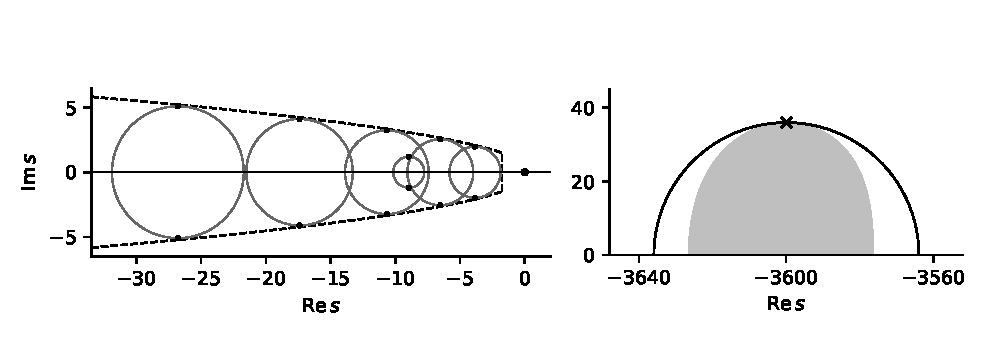
\includegraphics[width=\textwidth]{fig/pakes_disc.pdf}
\caption{Left: the sliver $\mathcal E_{T_0}$ of Theorem~\ref{bs:thm:local} for $T_0=2$ (dashed) and the discs $D_\gamma$ of six hypothetical zeros $a+ib$ with $a>2$ and $0<b<\frac12$, with the poles $-\gamma^2$ and $-\bar\gamma^2$ (dots) at the ends of their vertical diameters; the dot at $0$ marks the origin. Right: for the toy reciprocal Xi function with the first $200$ zeros of $\zeta$ and the pair $60\pm0.3i$, the set where $\Im\psi>0$ (shaded) on a grid of $481\times300$ points, which lies inside the upper half of $D_\gamma$ (solid); the cross is the pole $-\bar\gamma^2=-3599.91+36i$. Drawn by \texttt{pakes\_disc.py}.}
\label{bs:fig:disc}
\end{figure}

The threshold $p_*$ of Theorem~\ref{bs:thm:power} can be followed along the de Bruijn Newman flow. With $H_t$ and $\varphi_t(s)=H_t(0)/H_t(2i\sqrt s)$ as in Section~\ref{bh:sec:main}, so that $\varphi_0=\varphi$, let $\delta_*(t)$ be the largest angle $|\arg z|$ over the zeros $z$ of $H_t$ with $\Re z>0$, and $p_*(t)=1-2\delta_*(t)/\pi$. The proof of Theorem~\ref{bs:thm:power} uses only the product over the zeros, positivity on $(0,\infty)$ and the bound $|\arg z|<\pi/4$ required by Lemma~\ref{bs:lem:pair}, so whenever the zeros of $H_t$ satisfy that bound, $\varphi_t(x^p)$ is HCM if and only if $|p|\le p_*(t)$. By de Bruijn \cite{deBruijn} and Newman \cite{Newman1976} (Corollary~\ref{bh:cor:dbn}), $p_*(t)=1$ exactly for $t\ge\Lambda$; by Rodgers and Tao \cite{RodgersTao}, $p_*(t)<1$ for every $t<0$.

\begin{question}\label{bs:q:four}
Describe $p_*(t)=1-\frac2\pi\delta_*(t)$ for $t<0$. By Rodgers and Tao $p_*(t)<1$ for every $t<0$. Assume RH; how fast does $1-p_*(t)\to0$ as $t\uparrow0$?
\end{question}

Heuristically, the off line zeros of $H_t$ for small $|t|$ come from nearly coincident pairs of real zeros: by the isolated pair estimate of Section~\ref{ch:dbn}, a pair at distance $D_0$ collides near $t=-D_0^2/8$ and then has imaginary parts of order $\sqrt{|t|}$, at heights where the gap is of order $\sqrt{|t|}$. Since $1-p_*(t)$ is governed by $\max\Im z/\Re z$, the answer depends on the lowest height at which such a pair has collided, and so on the small gap statistics of the zeros. Both ingredients of an estimate are missing: de Bruijn's bound on the imaginary parts of the zeros runs only forward in time, from $H_0$ to $H_t$ with $t>0$, and no lower bound is known for the heights of the pairs that have collided by time $t$.

\subsection{The Thorin measure of $\varphi(s^p)$ and Bosch's variable}\label{bs:sec:thorin}

By Bondesson's theorem \cite[Theorem 6.1.1]{Bondesson}, a function with value $1$ at $0$ is HCM exactly when it is the Laplace transform of a GGC, so Theorem~\ref{bs:thm:power} already makes $\varphi(s^p)$ a GGC transform for $0<p\le p_*$.

\begin{theorem}\label{bs:thm:ggc}
Let $0<p\le p_*$. Then $\varphi(s^p)=\E e^{-sX_p}$ for a GGC variable $X_p$ with no drift. If $p<p_*$, its Thorin measure has the density
\begin{equation}\label{bs:eq:up}
u_p(\tau)=\frac{p}{\pi\tau}\,\Im\,\varepsilon_\varphi\bigl(\tau^pe^{ip\pi}\bigr)
=\frac{p}{2\pi\tau}\,\Im\Bigl[z\,\frac{\xi'}{\xi}\Bigl(\frac12+z\Bigr)\Bigr]_{z=\tau^{p/2}e^{ip\pi/2}}\ \ge0,\qquad\tau>0,
\end{equation}
which in terms of the zeros is
\begin{equation}\label{bs:eq:upzeros}
u_p(\tau)=\frac{p}{\pi\tau}\sum_\gamma\Im\frac{\tau^pe^{ip\pi}}{\tau^pe^{ip\pi}+\gamma^2}.
\end{equation}
If $p=p_*$, its Thorin measure is $u_{p_*}(\tau)\,d\tau$ plus a unit atom at $|\gamma|^{2/p_*}$ for every zero $\gamma$ with $\arg\gamma=-\delta_*$, counted with multiplicity, that is, one atom for each conjugate pair of zeros at the extreme angle; when $p_*=1$ there is an atom at $\gamma^2$ for every zero, and $u_1=0$.
\end{theorem}

\begin{proof}
Let $h=h_p$ and $\varepsilon_h(x)=p\,\varepsilon_\varphi(x^p)$. By the proof of Theorem~\ref{bs:thm:power}, $\varepsilon_h$ is analytic on $\Om$ and Pick. On $(0,\infty)$ it is nonnegative: a real zero contributes $x^p/(x^p+\gamma^2)>0$ and a pair contributes $2\Re\frac{s}{s+\varrho^2e^{2i\delta}}=\frac{2s(s+\varrho^2\cos2\delta)}{|s+\varrho^2e^{2i\delta}|^2}>0$. Hence $\varepsilon_h$ is complete Bernstein and $\varepsilon_h(x)/x=-(\log h)'(x)$ is a Stieltjes function, $a/x+b+\int U(dt)/(x+t)$. Here $a=\varepsilon_h(0+)=0$ and $b=\lim_{x\to\infty}\varepsilon_h(x)/x=0$ because $\varepsilon_\varphi(s)=O(\sqrt s\log s)$. Integrating from $0$ with $h(0)=1$ gives $h(x)=\exp(-\int\log(1+x/t)U(dt))$, a GGC transform. For $p<p_*$ the function $\varepsilon_h$ is continuous up to the upper edge of the cut, and Stieltjes inversion at $x=\tau e^{i\pi}$ gives $U(d\tau)=u_p(\tau)d\tau$ with $u_p(\tau)=\frac1{\pi\tau}\Im\varepsilon_h(\tau e^{i\pi})$, which is~\eqref{bs:eq:up};~\eqref{bs:eq:upzeros} follows from the Hadamard form of $\varepsilon_\varphi$. For $p=p_*$ the same inversion applies away from the points $x_0=\tau_0e^{i\pi}$ with $\tau_0=|\gamma|^{2/p_*}$ and $\arg\gamma=-\delta_*$, at which $x_0^{p_*}=-\gamma^2$. Near such a point the term of $\gamma$ in $\varepsilon_h$ is $p_*x^{p_*}/(x^{p_*}+\gamma^2)=x_0/(x-x_0)+O(1)$, so $\varepsilon_h(x)/x=1/(x+\tau_0)+O(1)$, and inversion gives a unit atom at $\tau_0$. On the ray itself this term equals $p_*\tau^{p_*}/(\tau^{p_*}-|\gamma|^2)$, which is real, so $u_{p_*}$ does not see the atom.
\end{proof}

\begin{corollary}\label{bs:cor:lamperti}
Let $L_p=Z_p/\tilde Z_p$ be the ratio of independent positive $p$ stable variables, whose density $\frac{\sin p\pi}{\pi}\,\frac{t^{p-1}}{t^{2p}+2t^p\cos p\pi+1}$ is Lamperti's \cite{boLamperti}; its power $L_p^{\,p}$ is Bosch's variable $T_\alpha$ with $\alpha=p$. Under RH the Thorin measure of $X_p$ is
\[
U_p=p\sum_\gamma\mathcal L\bigl(\gamma^{2/p}L_p\bigr),
\]
and $X_p\stackrel{d}{=}S_p\,X^{1/p}$, where $X=\sum_\gamma e_\gamma/\gamma^2$ is the clock variable of Proposition~\ref{prop:rigid}, with independent standard exponential variables $e_\gamma$, and $S_p$ is a positive $p$ stable variable independent of $X$ with $\E e^{-\lambda S_p}=e^{-\lambda^p}$. At $p=1/2$, $L_{1/2}\stackrel{d}{=}C^2$ for a standard Cauchy variable $C$, and $U_{1/2}=\frac12\sum_\gamma\mathcal L(\gamma^4C^2)$. As $p\uparrow1$, $L_p\to1$ and $U_p\to\sum_\gamma\delta_{\gamma^2}$ vaguely, the Thorin measure of $\varphi$ itself.
\end{corollary}

\begin{proof}
For real $\gamma$ the term of~\eqref{bs:eq:upzeros} equals $\frac{p}{\pi}\,\frac{\gamma^2\tau^{p-1}\sin p\pi}{\tau^{2p}+2\gamma^2\tau^p\cos p\pi+\gamma^4}$; substituting $\tau=\gamma^{2/p}t$ turns it into $p$ times Lamperti's density in $t$. The subordination identity is $\E e^{-sS_pY}=\E e^{-s^pY^p}$ with $Y=X^{1/p}$.
\end{proof}

Bosch's variable is therefore the kernel of the Thorin measure of $\varphi(s^p)$. Formula~\eqref{bs:eq:up} makes sense whatever the zeros are, and RH is the statement that it stays nonnegative as $p$ increases to $1$ (Question~\ref{bs:q:one} and the argument after it).

\begin{corollary}\label{bs:cor:rhX}
RH holds if and only if $X_p$ exists, that is $\varphi(s^p)$ is a GGC transform, for every $p\in(0,1)$. Unconditionally $X_p$ exists for $0<p\le1-1/(\pi T_0)$, in particular for $0<p\le1-1.1\times10^{-13}$, with the Thorin density~\eqref{bs:eq:up}.
\end{corollary}

\begin{proof}
If RH fails, $p_*<1$, and for $p\in(p_*,1)$ the function $\varphi(s^p)$ has a pole in $\Om$, which no GGC transform can have, since $\exp(-bs-\int\log(1+s/t)U(dt))$ is analytic and zero free on $\Om$. The rest is Theorem~\ref{bs:thm:ggc} with Corollary~\ref{bs:cor:uncond}, which gives $1-1/(\pi T_0)<p_*$.
\end{proof}

\begin{question}\label{bs:q:five}
Construct $X_{1/2}$ from Brownian motion, Bessel processes or the Biane, Pitman and Yor variables \cite{BPY01} without reference to the zeros. A construction that survived $p\uparrow1$ would prove RH by Corollary~\ref{bs:cor:rhX}.
\end{question}

\subsection{Positivity of the Thorin density from the primes}\label{bs:sec:open}

\label{bs:sec:limits}The method reads the threshold off the zeros: the elasticity has nonnegative imaginary part termwise on the sector $0<\arg s<\pi-2\delta_*$, and no information about $\delta_*$ is produced. A proof of RH along these lines must show $u_p\ge0$ for every $p<1$ directly from~\eqref{bs:eq:up}, for instance from the P\'olya kernel, from the prime sum of Remark~\ref{bs:rem:primes} or from a probabilistic model; this is the Thorin measure form of the reciprocal Xi programme of \cite{P17}. It cannot be done factor by factor: only the combination $(s-\frac14)\zeta(\frac12+\sqrt s)$ can enter an HCM or Pick argument (Section~\ref{bh:sec:use}).

\begin{question}\label{bs:q:one}
Prove $u_p\ge0$ for every $p\in(0,1)$ directly from~\eqref{bs:eq:up}, without locating the zeros.
\end{question}

The statement for all $p\in(0,1)$ is equivalent to RH. Under RH it holds by Theorem~\ref{bs:thm:ggc}. Conversely, suppose RH fails, let $\gamma=\varrho e^{i\delta_*}$ be a zero of maximal angle, and let $p\in(p_*,1)$; formula~\eqref{bs:eq:up} still defines $u_p$, except at isolated poles, although it is no longer a Thorin density. At $\tau=\varrho^{2/p}$ the term of $\bar\gamma$ in~\eqref{bs:eq:upzeros} equals $-\frac{p}{2\pi\tau}\cot\frac{\pi(p-p_*)}2$, which tends to $-\infty$ as $p\downarrow p_*$. The sum of the other terms stays bounded, because the other points $-\gamma'^2$ keep a positive distance from $-\bar\gamma^2$ and the tail of the sum is $O(\sum|\gamma'|^{-2})$. So $u_p$ takes negative values for $p$ slightly above $p_*$.

Along the ray write $\vartheta=p\pi/2\in(0,\pi/2)$, $t=\tau^{p/2}$, $z=te^{i\vartheta}$ and $w=\frac12+z$, so that $u_p(\tau)=\frac{p}{2\pi\tau}\Im[z\,\frac{\xi'}{\xi}(w)]$ by~\eqref{bs:eq:up}, and split $\xi'/\xi=\Gamma_\xi+\zeta'/\zeta$, where
\[
\Gamma_\xi(w)=\frac1w+\frac1{w-1}-\frac{\log\pi}2+\frac12\psi\Bigl(\frac w2\Bigr)
\]
is the logarithmic derivative of the factor $\frac12w(w-1)\pi^{-w/2}\Gamma(w/2)$ of $\xi$, and $\psi=\Gamma'/\Gamma$ is the digamma function, not the function $\psi$ of Theorem~\ref{bh:thm:main}. The ray crosses the critical strip for $t<t_e=1/(2\cos\vartheta)$ and then enters $\Re w>1$.

\begin{remark}[primes]\label{bs:rem:primes}
For $t>t_e$, that is $\tau>(2\cos(p\pi/2))^{-2/p}$, we have $\Re w>1$ and
\[
u_p(\tau)=\frac{p}{2\pi\tau}\Im\Bigl[z\Bigl(\frac1w+\frac1{w-1}-\frac{\log\pi}{2}+\frac12\psi\Bigl(\frac w2\Bigr)\Bigr)\Bigr]-\frac{p}{2\pi\tau}\sum_{n\ge2}\frac{\Lambda(n)}{\sqrt n}\,\Im\bigl(z\,n^{-z}\bigr),
\]
with $\Lambda$ the von Mangoldt function.
\end{remark}

\begin{proposition}\label{bs:prop:prime}
Let $\Re w>1$ and $\sigma=\Re w$. Then
\begin{equation}\label{bs:eq:primebound}
\frac{2\pi\tau}{p}\,u_p(\tau)\ \ge\ m_p(t):=\Im\Bigl[z\Bigl(\frac1{2w}+\frac1{w-1}+\frac12\log\frac{w}{2\pi}\Bigr)\Bigr]-\frac{t}{6\sigma^2}-t\Bigl(-\frac{\zeta'}{\zeta}\Bigr)(\sigma).
\end{equation}
Every term of $m_p$ is explicit, no zero of $\zeta$ enters, and $m_p(t)=\frac t2\sin\vartheta\log t\,(1+o(1))$ as $t\to\infty$. Consequently for each $p\in(0,1)$ there is $\tau_1(p)<\infty$ with $u_p(\tau)>0$ for all $\tau>\tau_1(p)$.
\end{proposition}

\begin{proof}
Binet's formula \cite[(5.9.13)]{DLMF} gives, for $\Re x>0$, $\psi(x)=\log x-\frac1{2x}-\int_0^\infty b(u)e^{-xu}du$ with $b(u)=\frac1{e^u-1}-\frac1u+\frac12\in[0,u/12]$. Hence $\psi(x)=\log x-\frac1{2x}-R$ with $|R|\le\frac1{12(\Re x)^2}$. With $x=w/2$ this turns $\Gamma_\xi(w)$ into $\frac1{2w}+\frac1{w-1}+\frac12\log\frac w{2\pi}-\frac R2$ with $|R|\le\frac1{3\sigma^2}$, so $\Im[z\Gamma_\xi(w)]$ is at least the first term of $m_p$ minus $t/(6\sigma^2)$. For the prime part, $\Im[z\,\zeta'/\zeta(w)]=-\sum\Lambda(n)\Im(zn^{-w})\ge-t\sum\Lambda(n)n^{-\sigma}$. The asymptotic follows from $\Im[z\log z]=t(\sin\vartheta\log t+\vartheta\cos\vartheta)$ and $-\zeta'/\zeta(\sigma)\to0$ as $\sigma\to\infty$.
\end{proof}

Table~\ref{bs:tab:prime} gives the point beyond which $m_p>0$, computed on a logarithmic grid of 50 points per decade, with $-\zeta'/\zeta(\sigma)$ evaluated directly. The entry $t_1$ is the last grid point at which $m_p\le0$, so the sign change lies within one grid step, a factor $10^{1/50}$, above it. These values are computed, not proved: nothing controls $m_p$ between grid points or beyond the last one.

The prime term of $m_p$ can be made elementary, because $-\zeta'/\zeta(\sigma)<1/(\sigma-1)$ for every $\sigma>1$. Delange \cite[Th\'eor\`eme]{Delange87} proves the sharper bound $-\zeta'/\zeta(\sigma)<1/(\sigma-1)-1/(2\sigma^2)$. Since $-\zeta'/\zeta(\sigma)$ enters $m_p$ with the factor $-t<0$, replacing it by $1/(\sigma-1)$ lowers $m_p$, and \eqref{bs:eq:primebound} still holds.

\begin{table}[h]
\centering
\begin{tabular}{ccccc}
\toprule
$p$ & strip exit $t_e=\frac1{2\cos\vartheta}$ & $t_1$ & $t_1/t_e$ & $\tau_1=t_1^{2/p}$\\
\midrule
$0.5$ & $0.707$ & $4.07$ & $5.75$ & $274$\\
$0.9$ & $3.20$ & $11.1$ & $3.47$ & $210$\\
$0.99$ & $31.8$ & $69.6$ & $2.19$ & $5.29\times10^3$\\
$0.999$ & $318$ & $553$ & $1.74$ & $3.10\times10^5$\\
$0.9999$ & $3183$ & $4818$ & $1.51$ & $2.33\times10^7$\\
\bottomrule
\end{tabular}
\caption{Where the lower bound~\eqref{bs:eq:primebound} becomes positive. On a logarithmic grid from $t_e$ to about $10^{14}t_e$, $m_p(t)>0$ at every grid point $t>t_1$; the ray reaches $t_1$ at $\tau_1=t_1^{2/p}$. The entries are computed, not proved.}
\label{bs:tab:prime}
\end{table}

\begin{remark}
The ratio $t_1/t_e$ tends to $1$. Near $\vartheta=\pi/2$ write $\sigma=1+x$, so $t=t_e(1+2x)$. The dominant terms of $m_p/t$ are $\frac12\log\frac t{2\pi}$ and $-\frac1x$, so positivity begins at $x\approx2/\log(t_e/2\pi)$, that is $t_1(p)=t_e(p)\bigl(1+\frac{4+o(1)}{\log(t_e/2\pi)}\bigr)$.
\end{remark}

So Question~\ref{bs:q:one} reduces, for each $p$, to the segment $|z|\le t_1(p)$ of the ray, which is asymptotically the part inside the critical strip. That part has length $t_e=1/(2\cos(p\pi/2))\approx1/(\pi(1-p))$, so heights and exponents correspond through $1-p\approx1/(\pi T)$, as in Corollary~\ref{bs:cor:uncond}.

\subsection{The density level and natural boundaries}

A variable with an HCM density is a GGC and so has an HCM Laplace transform ((F5) and (F6) of Section~\ref{bh:sec:bosch}). Under RH the clock variable $X=\sum_\gamma e_\gamma/\gamma^2$ is the GGC with transform $\varphi$. Its Cauchy counterpart is $X_C=\sum_ke_k/(2k-1)^2$, with transform $\sech(\pi\sqrt s/2)$.

\begin{theorem}\label{bs:thm:eta}
The density of $X_C$ is
\[
f_C(t)=\frac4\pi\sum_{k\ge1}(-1)^{k-1}(2k-1)e^{-(2k-1)^2t}=\frac4\pi\,\eta\Bigl(\frac{4it}{\pi}\Bigr)^3,\qquad t>0,
\]
with $\eta$ the Dedekind eta function. The line $\Re t=0$ is a natural boundary of $f_C$. Hence $X_C$ is a GGC whose Laplace transform is HCM, but the density of $X_C$ is not HCM.
\end{theorem}

\begin{proof}
The residue of $\sech(\pi\sqrt s/2)$ at $s=-(2k-1)^2$ is $\frac4\pi(-1)^{k-1}(2k-1)$, which gives the series once the Bromwich contour is moved to the left across the circles $|s|=4k^2$: for $s=4k^2e^{i\theta}$, $|\cosh(\pi\sqrt s/2)|^2=\sinh^2(\pi k\cos\frac\theta2)+\cos^2(\pi k\sin\frac\theta2)$ is at least $\frac14$ for every $\theta$ and at least $\sinh^2(\pi k/2)$ for $|\theta|\le2\pi/3$, while $|e^{st}|\le e^{-2k^2t}$ for $2\pi/3\le|\theta|\le\pi$, so for $t>0$ the integrals over the arcs of these circles to the left of the Bromwich line tend to $0$. Jacobi's identity $\eta(z)^3=\sum_{n\ge0}(-1)^n(2n+1)e^{\pi i(2n+1)^2z/4}$ \cite[Theorem 357]{boHardyWright}, at $z=4it/\pi$, where $e^{\pi i(2k-1)^2z/4}=e^{-(2k-1)^2t}$, gives the eta form. As a modular form $\eta$ has the real axis as natural boundary \cite[Chapter 11, Section 1.4, and Chapter 1, Section 4.2]{Remmert98}, and the real axis in $z$ is the line $\Re t=0$. An HCM density continues analytically to $\Om$ by~\eqref{bs:eq:bond}, so $f_C$ is not HCM.
\end{proof}

\begin{question}[density level]\label{bs:q:two}
Assume RH and that all zeros are simple. Does the density $f_X(t)=\sum_n A_n\gamma_n^2e^{-\gamma_n^2t}$ of $X$, with $A_n$ as in~\eqref{bh:eq:laplace}, have $\Re t=0$ as a natural boundary? If so, $X$ is not HCM.
\end{question}

P\'olya's gap theorem for Dirichlet series \cite{boPolya23,boPolya} says that if the exponents $\mu_n$ of a Dirichlet series $\sum_nc_ne^{-\mu_nt}$ have density $d=\lim n/\mu_n$ and satisfy $\inf_n(\mu_{n+1}-\mu_n)>0$, then every segment of length greater than $2\pi d$ on the line of convergence carries a singularity. When $\limsup\log n/\mu_n=0$ the abscissa of convergence equals $\limsup_n\log|c_n|/\mu_n$ \cite{boMandelbrojt}.

\begin{theorem}\label{bs:thm:nb}
Assume RH and that all zeros are simple, and assume
\begin{enumerate}
\item[(G)] $\inf_n(\gamma_{n+1}^2-\gamma_n^2)>0$;
\item[(D)] $\log\bigl(1/|\zeta'(\frac12+i\gamma_n)|\bigr)=o(\gamma_n^2)$.
\end{enumerate}
Then for $t>0$
\[
f_X(t)=\sum_nc_ne^{-\gamma_n^2t},\qquad c_n=A_n\gamma_n^2=-\frac{2\gamma_n\,\Xi(0)}{\Xi'(\gamma_n)},
\]
the series has abscissa of convergence $0$, and $\Re t=0$ is a natural boundary of $f_X$. In particular the density of $X$ is not HCM.
\end{theorem}

\begin{proof}
Residue expansion. The residue of $\varphi(s)=\Xi(0)/\Xi(i\sqrt s)$ at $s=-\gamma_n^2$ is $c_n$ as stated. Write $f_X$ as a Bromwich integral and move the contour to the left across the arcs of the circles $|s|=T_k^2$ that lie to the left of the Bromwich line, where, for large $k$, $T_k\in[k,k+1]$ is chosen at distance at least $c/\log k$ from every ordinate, with a small absolute constant $c>0$; this is possible because $[k-1,k+2]$ contains $O(\log k)$ ordinates \cite{HSW22}. Then $\zeta'/\zeta(\sigma+iy)=O(\log^2k)$ uniformly in $-1\le\sigma\le2$ and $|y-T_k|\le c/(2\log k)$ \cite[Theorem 9.6(A) and Section 14.4]{Titchmarsh}, and integration from $\sigma=2$ gives $1/|\zeta(\sigma+iy)|\le\exp(O(\log^2k))$ there. On the part of such an arc within angle $O(1/T_k)$ of the negative axis, $w=\frac12+\sqrt s$ has $\frac12\le\Re w\le2$ and $|\Im w|=\sqrt{T_k^2-(\Re w-\frac12)^2}=T_k+O(1/T_k)$, so for large $k$ it lies in this band or in its reflection in the real axis, and Stirling's formula gives $1/|\Xi(i\sqrt s)|\le\exp(O(T_k\log T_k))$, while $|e^{st}|\le e^{-tT_k^2/2}$. On the rest of the arc $\Re w\ge2$, and Stirling's formula gives $|e^{st}\varphi(s)|\le\exp\bigl(tT_k^2\cos\theta-\frac{T_k}2\cos\frac\theta2\log T_k+O(T_k)\bigr)$ for $s=T_k^2e^{i\theta}$. For $t>0$ both bounds tend to zero faster than any power of $T_k$, so the arcs contribute nothing in the limit and $f_X$ equals the residue series.

Abscissa. The exponents $\gamma_n^2$ satisfy $\log n/\gamma_n^2\to0$ and have density zero. By Stirling, $|\Xi'(\gamma_n)|=|\xi'(\rho_n)|=\gamma_n^{O(1)}e^{-\pi\gamma_n/4}|\zeta'(\rho_n)|$, so $\log|c_n|=\frac\pi4\gamma_n+O(\log\gamma_n)+\log(1/|\zeta'(\rho_n)|)$. Since $|\zeta'(\rho_n)|\le\gamma_n^{O(1)}$ always, (D) gives $\log|c_n|/\gamma_n^2\to0$, so the abscissa of convergence is $0$.

Natural boundary. By (G) and density zero, P\'olya's theorem places a singularity in every segment of the imaginary axis. An HCM density continues analytically to $\Om$, which contains the imaginary axis minus the origin.
\end{proof}

The same argument, with $\mu_k=(2k-1)^2$, gaps $8k$ and $c_k=\frac4\pi(-1)^{k-1}(2k-1)$, gives a second proof of Theorem~\ref{bs:thm:eta} that does not use modularity: by P\'olya's gap theorem \cite{boPolya23,boPolya} the line $\Re t=0$ is a natural boundary of $f_C$.

\begin{remark}[status of the hypotheses]
Hypothesis (D) is far weaker than the conjectured polynomial lower bounds for $|\zeta'(\rho)|$. Hypothesis (G) asks $\gamma_{n+1}-\gamma_n\ge c_0/(\gamma_n+\gamma_{n+1})$ for some $c_0>0$, a gap of order $1/\gamma$ against a mean spacing of order $1/\log\gamma$. Under the GUE model the expected number of violations is $\sum_n(\log\gamma_n/\gamma_n)^3<\infty$, so by the Borel Cantelli heuristic (G) fails at most finitely often, and then holds with a smaller $c_0$ if the zeros are simple.
\end{remark}

Numerically, for the first 200 zeros the coefficients $c_n$ computed from $\Xi'(\gamma_n)$ alternate in sign without exception; $\log|c_n|/\gamma_n^2$ equals $0.0462$, $0.0144$, $0.00524$, $0.00322$, $0.00195$ at $n=1,10,50,100,200$, tracking $\pi/(4\gamma_n)$; and the smallest gap $\gamma_{n+1}^2-\gamma_n^2$ is $159$, at $n=4$. The $c_n$ are the residues of the spectral expansion of the clock density in Section~\ref{ch:clocklaw}, written $R_k$ there, and Theorem~\ref{bs:thm:nb} describes, under its hypotheses, why that expansion cannot be continued past $t=0$.

For small $p$ the density of $X_p$ escapes this obstruction. The transform $\varphi(s^p)$ is analytic on the wider sector $|\arg s|<(\pi-2\delta_*)/p$ and, by Stirling's formula applied to $\xi(\frac12+z)$ for $|\arg z|<\pi/2$, decays along every ray strictly inside it. The inverse Laplace transform then continues the density of $X_p$ to the sector $|\arg t|<(\pi-2\delta_*)/p-\pi/2$, which contains $\Om$ when $p\le2p_*/3$.

\begin{question}\label{bs:q:three}
Determine $\{p:\ X_p\ \text{is HCM}\}$, and the same set for the Cauchy family $X_{C,p}$ with transform $\sech(\pi s^{p/2}/2)$.
\end{question}

Two facts constrain the answer. Under RH, $X_p\stackrel{d}{=}S_pX^{1/p}$, and positive $p$ stable variables are HCM exactly for $p\le1/2$, a conjecture of Bondesson \cite[Sections 5.7, 5.8 and 7.2]{Bondesson} proved by Bosch and Simon \cite[p.~32]{BoschSimon16}. Since HCM is preserved under products of independent variables and under powers of modulus at least one ((F1) and (F2) of Section~\ref{bh:sec:bosch}), HCM of $X$ would give HCM of $X_p$ for $p\le1/2$; but Theorem~\ref{bs:thm:nb} shows that $X$ is not HCM under (G) and (D), so this route is closed unless those hypotheses fail. The elasticity criterion reduces Question~\ref{bs:q:three} to the absence of zeros of the density $f$ of $X_p$ in $\Om$ and the Pick property of $-tf'(t)/f(t)$; by the continuation argument before Question~\ref{bs:q:three}, $f$ is at least analytic on $\Om$ for small $p$. A numerical scan of this elasticity for $X_{C,1/2}$ would be the first test.

\subsection{The Mellin variable $W$ and the first gap}

Question~\ref{bh:q:beta} asks for which $\beta$ the density of $W^\beta$ is HCM; on the Cauchy side the answer is $|\beta|\ge2$. Let $\chi(t)=\xi(\frac12)/\xi(\frac12+t)=\prod_\gamma(1+t^2/\gamma^2)^{-1}$ and let $g(y)=\frac1\pi\int_0^\infty\chi(t)\cos(ty)\,dt$ be the function $g$ of Section~\ref{bh:sec:dict}, which is entire because $\chi(t)=\exp(-\frac12|t|\log|t|(1+o(1)))$. By the van Dantzig pair of Section~\ref{ch:clock}, recalled in Section~\ref{bh:sec:dict}, $\chi$ is a characteristic function without RH: the clock variable $T$ exists unconditionally \cite[Theorem A]{P26}, and if $Z$ is a standard normal variable independent of $T$ then $\E e^{itZ\sqrt{2T}}=\E e^{-t^2T}=\chi(t)$. So $g$ is the density of the normal scale mixture $Z\sqrt{2T}$, and $W=\exp(Z\sqrt{2T})$ exists without any hypothesis. By the elasticity criterion, HCM of $W^\beta$ becomes a sign condition on $-g'/g$ in a strip (Proposition~\ref{bs:prop:Wcrit}), and since $g$ is entire no natural boundary stands in the way.

\subsubsection{A lower bound for $g$}

Theorem~\ref{bs:thm:gpos} proves the existence of $W$ a second time, independently of \cite[Theorem A]{P26}.

\begin{theorem}\label{bs:thm:gpos}
Unconditionally, by the verification of RH to height $T_0$ \cite{PT21}, $g(y)\ge0.9998\,g_R(y)>0$ for all real $y$, where $g_R$ is the density of $\sum_{\gamma\ \mathrm{real}}L_\gamma/\gamma$. Hence $\chi$ is a characteristic function and there is a positive random variable $W$ with $\E W^{it}=\chi(t)$ and $\E W^z=\Xi(0)/\Xi(z)$ for $|\Re z|<\gamma_1$.
\end{theorem}

\begin{proof}
Split $\chi=\chi_R\chi_{\mathrm{off}}$ into the products over real zeros and over conjugate pairs of nonreal zeros. For a pair $\gamma=\varrho e^{i\delta}=a+ib$ with $a,b>0$, the factor $(1+t^2/\gamma^2)^{-1}(1+t^2/\bar\gamma^2)^{-1}$ is the Fourier transform of the even kernel
\[
k_\gamma(x)=\frac{\varrho}{2\sin2\delta}\,e^{-a|x|}\sin(b|x|+\delta),
\]
of total mass one, positive for $|x|<(\pi-\delta)/b$ and bounded by $\frac{\varrho}{2\sin2\delta}e^{-a|x|}$. List the pairs as $\gamma^{(1)},\gamma^{(2)},\ldots$ in order of $\Re\gamma$, write $k_j=k_{\gamma^{(j)}}$, and let $\chi_m$ be the product of the first $m$ pair factors, $\nu_m=k_1*\cdots*k_m$ and $g_m=g_R*\nu_m$, the function with Fourier transform $\chi_R\chi_m$. We bound $g_m$ uniformly in $m$ and let $m$ grow at the end.

Comparison. $g_R=\ell*\tilde g_R$, where $\ell(z)=\frac{\gamma_1}2e^{-\gamma_1|z|}$ is the density of $L_{\gamma_1}/\gamma_1$ and $\tilde g_R$ is the density of the sum over the other real zeros, so $e^{-\gamma_1|x|}g_R(y)\le g_R(y-x)\le e^{\gamma_1|x|}g_R(y)$. Writing $\nu_m=\nu_m^+-\nu_m^-$,
\[
g_m(y)\ge g_R(y)\Bigl(\int e^{-\gamma_1|x|}\nu_m(x)dx-2\int\cosh(\gamma_1x)\,\nu_m^-(x)dx\Bigr)=:g_R(y)(A_m-2B_m).
\]

The term $A_m$. By Parseval, $A_m=\frac1\pi\int\chi_m(t)\frac{\gamma_1}{\gamma_1^2+t^2}dt=\E\,\chi_m(\gamma_1C)$ with $C$ a standard Cauchy variable. For $s\ge0$ each pair factor is $|1+s/\gamma^2|^{-2}\ge(1+s/\varrho^2)^{-2}\ge e^{-2s/\varrho^2}$, so $A_m\ge\E e^{-\kappa C^2}=e^\kappa\operatorname{erfc}(\sqrt\kappa)$ with $\kappa=2\gamma_1^2\Sigma_{\mathrm{off}}$ and $\Sigma_{\mathrm{off}}=\sum_{\mathrm{off}}|\gamma|^{-2}$. All nonreal zeros have $\Re\gamma>T_0=3\times10^{12}$ \cite{PT21}, so with $N(T)\le T\log T$ for $T\ge T_0$, $\Sigma_{\mathrm{off}}\le2\int_{T_0}^\infty N(T)T^{-3}dT\le2(\log T_0+1)/T_0<2\times10^{-11}$, $\kappa<8\times10^{-9}$ and $A_m>0.99989$.

The term $B_m$. For even signed measures $\int\cosh(\gamma_1x)\,d(|\mu|*|\nu|)=\int\cosh(\gamma_1 x)d|\mu|\cdot\int\cosh(\gamma_1x)d|\nu|$ exactly, and $(\mu*\nu)^-\le\mu^+*\nu^-+\mu^-*\nu^+$. Hence, with $M(\cdot)=\int\cosh(\gamma_1x)\,d(\cdot)$ and since $M(|k_\gamma|)\ge M(k_\gamma)=|1-\gamma_1^2/\gamma^2|^{-2}\ge1$,
\[
B_m\le\sum_{j\le m}M(k_j^-)\prod_{i\le m,\ i\ne j}M(|k_i|)\le SP,\qquad S=\sum_\gamma M(k_\gamma^-),\quad P=\prod_\gamma M(|k_\gamma|),
\]
with the sum and the product over all pairs. Here $k_\gamma^-$ lives on $|x|\ge(\pi-\delta)/b$ and $M(k_\gamma^-)\le\frac{\varrho}{\sin2\delta\,(a-\gamma_1)}\exp\bigl(-(a-\gamma_1)\frac{\pi-\delta}{b}\bigr)$. As $\varrho/\sin2\delta=\varrho^3/(2ab)$, this bound is $\frac{\varrho^3}{2a(a-\gamma_1)}\,b^{-1}e^{-K/b}$ with $K=(a-\gamma_1)(\pi-\delta)$. For fixed $a$ it increases with $b$: $\varrho$ increases, $K$ decreases because $\delta=\arctan(b/a)$ increases, and $b\mapsto b^{-1}e^{-K/b}$ increases on $(0,K)$. So, as $b<\frac12$, it is at most
\[
F(a)=\frac{(a^2+\frac14)^{3/2}}{a(a-\gamma_1)}\exp\Bigl(-2(a-\gamma_1)\bigl(\pi-\arctan\tfrac1{2a}\bigr)\Bigr),
\]
and $F(T_0)<\exp(-1.88\times10^{13})$, while $-(\log F)'>6$ on $[T_0,\infty)$. Every pair has $a>T_0$, so Stieltjes integration against $N(T)\le T\log T$ gives
\[
S\le F(T_0)\Bigl(T_0\log T_0+\frac{\log T_0+1}6+\frac1{36T_0}\Bigr)<\exp(-1.8\times10^{13}).
\]
Moreover $M(|k_\gamma|)=M(k_\gamma)+2M(k_\gamma^-)$ and $M(k_\gamma)\le\exp(3\gamma_1^2/\varrho^2)$, so $\log P\le3\gamma_1^2\Sigma_{\mathrm{off}}+2S<1.2\times10^{-8}$. So $A_m-2B_m>0.9998$ for every $m$.

Limit. For real $t$ each pair factor lies in $(0,1]$, and $\chi_R$ is integrable because it contains the factor $(1+t^2/\gamma_1^2)^{-1}$. By dominated convergence in the Fourier inversion integral, $g_m\to g$ uniformly on $\R$, so $g\ge0.9998\,g_R$. The comparison also gives $g_m(y)\le g_R(y)\int e^{\gamma_1|x|}|\nu_m(x)|dx\le2P\,g_R(y)$, since $e^{\gamma_1|x|}\le2\cosh(\gamma_1x)$ and $|\nu_m|\le|k_1|*\cdots*|k_m|$, so $g\le2P\,g_R$. Hence $g$ is integrable, its Fourier transform is $\chi$, and $\chi(0)=1$ makes $g$ a probability density. Finally $\int e^{cy}g_R(y)dy=\prod_{\gamma\ \mathrm{real}}(1-c^2/\gamma^2)^{-1}<\infty$ for $|c|<\gamma_1$, so $\int e^{c|y|}g(y)dy<\infty$ there, $\E W^z=\int e^{zy}g(y)dy$ is analytic on $|\Re z|<\gamma_1$, and it equals $\Xi(0)/\Xi(z)$ there because the two agree on the imaginary axis.
\end{proof}

The proof uses only that the zeros with $0<\Re\gamma\le T_0$ are real. The pair kernel formula and the constants of the proof were also checked numerically (\texttt{code/\allowbreak README.md}).

\subsubsection{Which powers of $W$ are HCM}

For real $\beta\ne0$ the density of $W^\beta$ is $x^{-1}g(\log x/\beta)/|\beta|$. With $y=\log x$, its elasticity is $1-\frac1\beta\frac{g'}{g}(y/\beta)$, and $x\in\C^+$ corresponds to $0<\Im y<\pi$; for $\beta<0$ the point $u=y/\beta$ then lies in the lower half of the strip $|\Im u|<\pi/|\beta|$, where the factor $\frac1\beta<0$ reverses the sign condition, and $g(\bar u)=\overline{g(u)}$, as $g$ is real on $\R$, moves it to the upper half. Theorem~\ref{bs:thm:crit} therefore gives the following.

\begin{proposition}\label{bs:prop:Wcrit}
Let $\beta\in\R\setminus\{0\}$. Then $W^\beta$ is HCM if and only if $g$ has no zeros in the strip $|\Im u|<\pi/|\beta|$ and $\Im\bigl(-g'(u)/g(u)\bigr)\ge0$ for $0<\Im u<\pi/|\beta|$.
\end{proposition}

As $\Im u\downarrow0$ the condition requires $(\log g)''\le0$ on $\R$; numerically $(\log g)''\le-2.2$ on $[0,1]$. On the Cauchy side $g_C=1/(\pi\cosh u)$, $-g_C'/g_C=\tanh u$, which is Pick on $0<\Im u<\pi/2$ with a pole at $i\pi/2$; Proposition~\ref{bs:prop:Wcrit} gives $|\beta|\ge2$, Bosch's theorem once more.

\begin{theorem}\label{bs:thm:gap}
Assume RH, simple zeros, and $\log(1/|\zeta'(\rho_n)|)=O(\gamma_n)$. Then $u_0=\frac\pi4+\limsup_n\gamma_n^{-1}\log(1/|\zeta'(\rho_n)|)$ is finite, and for $\Re u>u_0$
\[
g(u)=-\Xi(0)\sum_n\frac{e^{-\gamma_nu}}{\Xi'(\gamma_n)}=\sum_nb_ne^{-\gamma_nu},\qquad b_1>0>b_2,
\]
and if $W^\beta$ is HCM then $|\beta|\ge\gamma_2-\gamma_1=6.8873\ldots$.
\end{theorem}

\begin{proof}
The expansion is the residue computation for the Fourier integral $g(u)=\frac1{2\pi}\int\chi(t)e^{-itu}\,dt$ closed in the lower half plane. We move the line of integration to $\Im t=-T_k$, where $T_k\in[k,k+1]$ are heights at which $1/\zeta(\sigma\pm iT_k)=T_k^{O(1)}$ uniformly in $-1\le\sigma\le2$ \cite[Theorem 9.7]{Titchmarsh}; by Stirling's formula and the functional equation the moved integral is $O(e^{(\pi/4-\Re u)T_k+O(\log T_k)})$, which tends to $0$ for $\Re u>\pi/4$, so there $g(u)$ is the limit of the sums of the residue terms over $\gamma_n<T_k$. By Stirling, $\log|b_n|=\frac\pi4\gamma_n+\log(1/|\zeta'(\rho_n)|)+O(\log\gamma_n)$, so the series converges absolutely for $\Re u>u_0$, and $u_0\ge\pi/4$ because $|\zeta'(\rho_n)|\le\gamma_n^{O(1)}$, so its sum is $g(u)$ there (conjecturally $u_0=\pi/4$); the signs come from $b_n=\frac{\gamma_n}2A_n$. Put $\Delta=\gamma_2-\gamma_1$. As $\Re u\to\infty$ with $\Im u=v$ fixed,
\[
\Im\Bigl(-\frac{g'}{g}\Bigr)(x+iv)=\Delta\Bigl|\frac{b_2}{b_1}\Bigr|e^{-\Delta x}\sin(\Delta v)\,\bigl(1+O(e^{-cx})\bigr),\qquad c>0.
\]
For $\pi/\Delta<v<2\pi/\Delta$ this is negative for large $x$. If $|\beta|<\Delta$ the strip $0<\Im u<\pi/|\beta|$ contains such $v$, and Proposition~\ref{bs:prop:Wcrit} fails.
\end{proof}

\begin{question}[first gap conjecture]\label{bs:q:gap}
Is $W^\beta$ HCM exactly when $|\beta|\ge\gamma_2-\gamma_1$? On the Cauchy side the analogous statement, with frequencies $2k-1$, is Bosch's theorem at $\alpha=1/2$: $3-1=2$.
\end{question}

With $b_n$ computed from $\Xi'(\gamma_n)$ ($b_1=359.52$, $b_2=-28007$, $b_3=392918$) and $g$ computed by quadrature near the origin, a scan of $4840$ points with $0\le x\le6$ and $0<v<0.99\,v_*$, where $v_*=\pi/\Delta=0.45614$, found no value of $\Im(-g'/g)$ below $-1.3\times10^{-15}$, which is rounding; in 40 digit arithmetic the minimum over $1.1\le x\le9.1$ at $v=0.999\,v_*$ is $+1.0\times10^{-27}$. Just above the threshold the sign flips: the minimum is $-6.5\times10^{-8}$ at $v=1.001\,v_*$, so numerically the threshold is sharp to $0.1$ per cent.

Proving sufficiency requires the Pick property of $-g'/g$ in the full strip $0<\Im u<\pi/\Delta$, which near the origin is a statement about the P\'olya type kernel $g$ that does not reduce to the zeros.

\subsubsection{Solvable models}

To see whether the first gap rule is a coincidence of the half Cauchy case, we test it on a family in which everything is explicit. The logistic variable $\log W$ has characteristic function $\pi t/\sinh(\pi t)=\prod_{k\ge1}(1+t^2/k^2)^{-1}$. Removing a finite set $R$ of frequencies multiplies the characteristic function by $\prod_{k\in R}(1+t^2/k^2)$, which gives $g=\prod_{k\in R}(1-D^2/k^2)L$ with $D=d/dy$ and $L(y)=\frac14\sech^2(y/2)$. For each model we locate numerically the largest strip on which $\Im(-g'/g)\ge0$; by Theorem~\ref{bs:thm:crit}, as in Proposition~\ref{bs:prop:Wcrit}, its width $h_*$ gives the HCM threshold $\beta_*=\pi/h_*$. Table~\ref{bs:tab:gaps} lists the results.

\begin{table}[h]
\centering
\begin{tabular}{llccc}
\toprule
frequencies & gaps & first gap & largest gap & $\beta_*=\pi/h_*$\\
\midrule
$1,2,3,\ldots$ & $1,1,1,\ldots$ & 1 & 1 & $1.000$\\
$1,3,5,\ldots$ (half Cauchy) & $2,2,2,\ldots$ & 2 & 2 & $2$ (Bosch)\\
$1,3,4,5,\ldots$ & $2,1,1,\ldots$ & 2 & 2 & $2.000$\\
$1,3,5,6,\ldots$ & $2,2,1,\ldots$ & 2 & 2 & $2.000$\\
$1,3,4,6,\ldots$ & $2,1,2,1,\ldots$ & 2 & 2 & $2.000$\\
$1,4,5,6,\ldots$ & $3,1,1,\ldots$ & 3 & 3 & $3.000$\\
$1,4,5,7,\ldots$ & $3,1,2,1,\ldots$ & 3 & 3 & $3.000$\\
$1,4,7,8,\ldots$ & $3,3,1,\ldots$ & 3 & 3 & $3.000$\\
$1,5,6,7,\ldots$ & $4,1,1,\ldots$ & 4 & 4 & $4.000$\\
$1,2,4,5,\ldots$ & $1,2,1,\ldots$ & 1 & 2 & $1.269$\\
$1,2,3,6,\ldots$ & $1,1,3,1,\ldots$ & 1 & 3 & $1.317$\\
$1,2,5,6,\ldots$ & $1,3,1,\ldots$ & 1 & 3 & $1.483$\\
\bottomrule
\end{tabular}
\caption{HCM threshold for powers of $W$ in logistic models with frequencies removed, computed as $\beta_*=\pi/h_*$ from the width $h_*$ of the largest strip on which $\Im(-g'/g)\ge0$. The half Cauchy row is Bosch's theorem, not a computation.}
\label{bs:tab:gaps}
\end{table}

Whenever the first gap is at least as large as every later gap, the computed threshold equals the first gap, to the resolution of the computation. When some later gap exceeds the first, the threshold lies strictly between the first gap and the largest gap, and depends on where the large gap sits. The asymptotic argument of Theorem~\ref{bs:thm:gap} explains the lower bound in all cases. For the Riemann zeros the first gap $\gamma_2-\gamma_1=6.8873$ exceeds every later gap among the first $1000$ zeros (the next largest is $\gamma_4-\gamma_3=5.414$). The explicit form of the Riemann von Mangoldt formula of Hasanalizade, Shen and Wong, $|N(T)-\frac T{2\pi}\log\frac T{2\pi e}-\frac78|\le2.5167+\frac1{50T}$ for $e\le T\le X_0=30\,610\,046\,000$ and $\le0.1095\log T+0.2042\log\log T+3.0305+\frac1{50T}$ for $T>X_0$ \cite[(1.7), (2.7) and Corollary~1.4]{HSW22}, shows that every interval $(T,T+6.887]$ with $T\ge1000$ contains an ordinate: the lower bound it gives for the number of ordinates there exceeds $0.52$ at $T=1000$, increases with $T$ while $T+6.887\le X_0$, and exceeds $11$ beyond. So every gap that starts above height $1000$ is at most $6.887$, less than the first, and every gap that starts below it is a gap between two of the first $650$ zeros, since $N(1000)=649$. The first gap therefore exceeds every later gap. This refines Question~\ref{bs:q:gap}.

\begin{question}[first gap conjecture, refined]\label{bs:q:gaprefined}
Let $Y=\sum_nL_n/\lambda_n$ with independent standard Laplace variables $L_n$ and $0<\lambda_1<\lambda_2<\cdots$, and let $W=e^Y$. If the characteristic function of $Y$ decays faster than every exponential, or if the first gap $\lambda_2-\lambda_1$ is at least every later gap, is the HCM threshold of $W^\beta$ exactly $\lambda_2-\lambda_1$? In particular, is it $\gamma_2-\gamma_1$ for the Riemann variable?
\end{question}

\subsection{Where the difficulty lies}\label{bs:sec:discussion}

Bosch's theorem cannot be the input to a proof that the reciprocal Xi function is HCM, because for a product over the zeros HCM is equivalent to the reality of the zeros (Proposition~\ref{bh:prop:closure}), and Section~\ref{ch:sato} finds that every GGC criterion in the books of Sato and Bondesson is, at the centre, equivalent to RH. Bosch's method does transfer: at each of three levels it isolates one concrete object on which the question turns.

At the level of transforms the object is the Thorin density $u_p$ of~\eqref{bs:eq:up}. Its positivity for every $p<1$ is equivalent to RH; the primes prove it on each ray beyond some point, that point is asymptotically where the ray leaves the critical strip, and what remains is a segment of length about $1/(\pi(1-p))$. The first direction is to prove positivity on that segment from the explicit formula for $\xi'/\xi$ rather than from the zeros; computation alone extends the unconditional range $p\le1-1/(\pi T_0)$ only as fast as the verification height $T_0$ grows.

At the level of the Mellin variable the object is the sign of $\Im(-g'/g)$ in the strip $0<\Im u<\pi/(\gamma_2-\gamma_1)$. The second direction is to prove the first gap conjecture, first in the logistic models of Table~\ref{bs:tab:gaps}, where every quantity is elementary, and then for $W$, whose threshold the scan after Question~\ref{bs:q:gap} already locates to $0.1$ per cent. Question~\ref{bh:q:single} remains open.

At the level of densities the object is the natural boundary. The third direction is to establish it for the clock variable without the hypotheses (G) and (D) of Theorem~\ref{bs:thm:nb}, which would show what replaces, on the Riemann side, the modularity that produces the natural boundary on the Cauchy side.

Section~\ref{ch:heat} approaches the Thorin functional $\sum_\gamma\delta_{\gamma^2}$ of the clock, its Thorin measure under RH, from the other end of Bondesson's hierarchy, through its Laplace transform, the heat trace $W(t)=\sum_\gamma e^{-\gamma^2t}$.
